% Paperformat
\documentclass[a4paper, 12pt]{scrartcl}
\usepackage{cite}
\usepackage{ragged2e}
\usepackage{url}
\usepackage{bm} % bold math
\usepackage{nccmath} % medium fraction with mfrac 
\usepackage{amssymb}
\usepackage{graphicx}
\usepackage{amsthm} % theorems
\usepackage{hyperref}
\usepackage{float}

\newtheorem{theorem}{Theorem}[section]
\begin{document}

\begin{titlepage}
	\vspace*{\stretch{1}}
	\begin{center}
		{\Large\bfseries Bachelor Thesis}           \\[6.5ex]
		
		{\huge\bfseries Visualizing Dynamic Programming on Tree Decompositions}                  \\[6.5ex]
		
		\vspace{6ex}
				
		\textsc{\Large Martin Röbke}    \\[3ex]
		{\Large born: 04.03.1995 in Dresden, Germany}    \\[2ex]
		{\Large matriculation number: 3949819}    \\[2ex]
		{\Large martin.roebke@tu-dresden.de}    \\[2ex]
		\textsc{\large 
			}             \\[12ex]
		\vfill
		{\Large Technische Universität Dresden}               \\
		Faculty of Computer Science \\
		International Center For Computational Logic 		\\[5ex]
		
		{\Large Supervisor: Dr. Johannes Fichte}\\[2ex]
		{\Large Second Referee:  Prof. Dr. rer. nat. Stefan Gumhold}\\[5ex]
		
		\vfill
		Dresden, \today
	\end{center}
	\vspace{\stretch{2}}
\end{titlepage}



\section*{Abstract}
\vspace{4ex}
The present Bachelor thesis is about a practical and lightweight implementation of visualizing dynamic programming on tree decompositions.
I created the python-package tdvisu for the purpose of visualizing, teaching and analyzing the solving process of MSOL-problems using dynamic programming.
As reference implementations of dynamic programming on tree decompositions the projects \href{https://github.com/daajoe/GPUSAT}{GPUSAT} and \href{https://github.com/hmarkus/dp_on_dbs}{dpdb} were chosen.

????????Who benefits from using

\newpage

%  table
\tableofcontents

% chapter on next page
\newpage


\section{Introduction}
intro. mit motivation und related work, state of the art, advancements.

Idee für Projekt 
Wen interessiert es?

Probleme bei Umsetzung

Neue Zielstellung

Visualization Pipeline

Stand Umsetzung, Tools

\newpage
\section{Background}
\subsection{MSOL}
\subsection{Tree Decomposition}
\subsection{Courcelle's Theorem}
\begin{quotation}
	Every graph property definable in monadic second-order logic (MSO) is decidable in linear time on graphs of bounded treewidth.\\
	{\small Courcelle, Bruno (1990)}\footnote{Courcelle, Bruno "The monadic second-order logic of graphs. I. Recognizable sets of finite graphs",\\ Information and Computation, 85 (1990) no. 1: 12-75}
\end{quotation}

For all $k \in \mathbb{N}$ and MSO-sentences F is the decision problem for a given graph G, whether $G \models F$ is true, in time $2^{p(tw(G))} \cdot |G|$ with a polynom p decidable.
\begin{itemize}
	
	\item \emph{drawback:} still expensive ($2^{p(tw G)}$, $2^{2^{(\#Q)}}$, large constants) \smallskip 

\end{itemize}

The workflow then looks like we see in figure~\ref{fig:UsageCourcelle}.

\begin{figure}[H]
	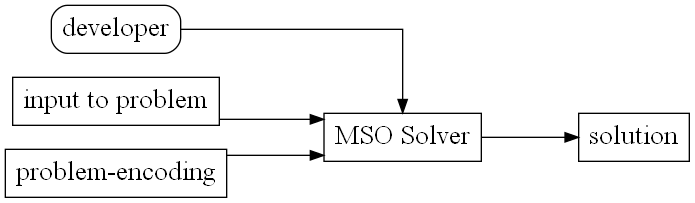
\includegraphics[height=0.2\textheight]{images/UsageCourcelle.gv.png}
	\caption{Implementation of the theorem}
	\label{fig:UsageCourcelle}
\end{figure}

\newpage
\section{Concept}
What I do and why I did it
\newpage
\section{My Visualization Project}
Trello
Github
Slack
Ziele
Stand 
Beispiele
Ausblick
\newpage
\subsection{Integration in GPUSAT}
Programm
Umsetzung
Beispiel
\newpage
\subsection{Integration in dpdb}
Programm
Umsetzung
Beispiel
\newpage
\section{Application and Images }
beispiele und ergebnisse das vertex cover eignet sich dafür hervoragend
Z.B. Fehler in VC <-> Visualization
\newpage
\section{Summary and Outline}

\bibliography{bibtex}{}
\bibliographystyle{ieeetr}

\end{document}